%************************************************
\chapter{X-ray diffraction and Polarimetry}
%************************************************
\begin{flushright}
November 8, 2012
\end{flushright}
\section{Objective}
To
	\begin{enumerate}
		\item observe and understand the X-ray diffraction technique
		\item use optical activity of a substance for concentration estimation
	\end{enumerate}

\section{Theory}
	\subsection{X-ray diffraction}
		The very fist condition for X-ray diffraction analysis of a substance is that it must crystallize. To check the quality of the crystal, a polarized beam of light is passed through it and using a microscope and an analyser (another polariser), the crystal is viewed. The colour must be the same for any given orientation of the analyser, if the crystal formed is good in terms of being analysed by this technique.
		For holding the crystal, nylon thread loops are used, with super-glue to fix them in place. This is then placed into the single crystal x-ray diffraction machine. There are various degrees of freedom in this device. $\kappa$ can range from $-90 ^o$ to $+90 ^o$ using an arm. The base can rotate $360 ^o$. The detector can move $2 \theta$, where $\theta$ depends on the detector being used. Also, the detector can move forward and backwards. Intenisty falls rapidly with distance. However, if the diffracted beams are at a very small angular difference, then distance helps resolve these. An optimal condition must be met to improve resolution at the cost of intensity. 
		The anode is required to be cooled constantly to create the X-ray. To produce higher intensities of X-rays, moving anodes are used, that helps dissipate the heat and thereby allows for higher power.
		The spots that are obtained, are first matched with a unit cell that's specified by the user. The unit cells can be mathematically shown to be limited.
		X-ray diffraction is a very strong tool as this is amongst the few analytic techniques that can be used to resolve the chirality of the molecule, which is essentially known if you can resolve the exact 3D-structure of the molecule, which is what is obtained after calculations using this technique. Once the spatial arrangement is known, the R and S classification can be done easily.
		The temperature is normally kept to the room temperature, but for more accurate results, the temperature can be dropped to avoid thermal energy induced errors.
		The machine also has a $CO_2$ laser which is used to analyse substances that crystallize at low temperatures only. The experimental setup is such that the laser is reflected and targeted using a combination of mirrors, atleast one of which is movable. Now the substance to be analysed is put in a thin high quality capillary tube which is sealed using a super-glue. Now the capillary is placed in the machine and cooled. The laser heats a small part of the wall of the capillary, which in turn heats the now frozen liquid inside back into a liquid. The laser moves upwards gradually, as slow as $3 cm$ in $2$ hours. This is similar to zone melting and it results in formation of a crystal. After the process is over, a single transparent frozen area is usually obtained, which is used for analysis. The rest of the area is also solid, but not transparent.
	\subsection{Polarimetry}
		Specific rotation is given by $\alpha=\theta/lc$, where $\theta$ is the angle by which the light is rotated, $l$ is the path length, and $c$ is the concentration given in moles per Litre.
		Optically active substances are those that rotate the plane of polarization of plane-polarized light. Before we get into understanding what that means, it's important to realise that refractive index of a medium, which essentially dictates the speed of light through the medium, is a function of the material's dipole properties. Having made that clear, let us now decompose our plane polarized light into two components, each consisting of a circularly polarised light, with one going clockwise and the other going anti-clockwise, suitably chosen to produce the plane polarized light, when added vectorially. Now if the molecule's environment is chiral, viz. the molecule is not a super-imposable  mirror image of itself, on itself\footnote {which more precisely may be stated as, only if it does not posess an axis of improper rotation, $S_n$}, and in a given mixture, there exists only one kind of molecule (say right handed using some arbitrary definition), then one of the circularly polarised light (say clockwise) will travel at a different rate than the anti-clockwise circularly polarised light and thereby when it leaves the medium, their superposition would result in a plane wave with a plane that's at an angle with the incident plane of the wave. An important question to address at this stage is that we're talking about molecules which are randomly oriented and what effect will this have on the discussion so far. A little thought reveals that the molecules with the chiral axis at some angle $\phi$ wrt the plane of light, are equally likely to be found as the molecules at an angle $-\phi$. Since the molecules are chiral, their contribution to the phase difference of the circularly polarised decomposition of the plane polarised light, will not average out to zero. It's the cumulative effect that we see. From this it's natural to consequence that the optical activity depends directly on the concentration of the molecule. Also, the phase difference will be larger if the light travels a longer distance inside the chiral medium, and thus optical activity depends on the 
		\par
		What we're doing in the experiment is essentially keeping the length constant and changing the concentration. If we plot the $\theta$ against the concentration, we will get $l\alpha$, which is constant for the given experiment.


\section{Observations/Discussion}
	\subsection{X-ray diffraction}
		There aren't any `observations' to report for this experiment as this experiment was demonstrated to us.
	\subsection{Polarimetry}
		Values and the graph for Relative Concentration vs. $\theta$ are given in \autoref{E11_optical}.

		\begin{figure}[bth]
			\begin{center}
				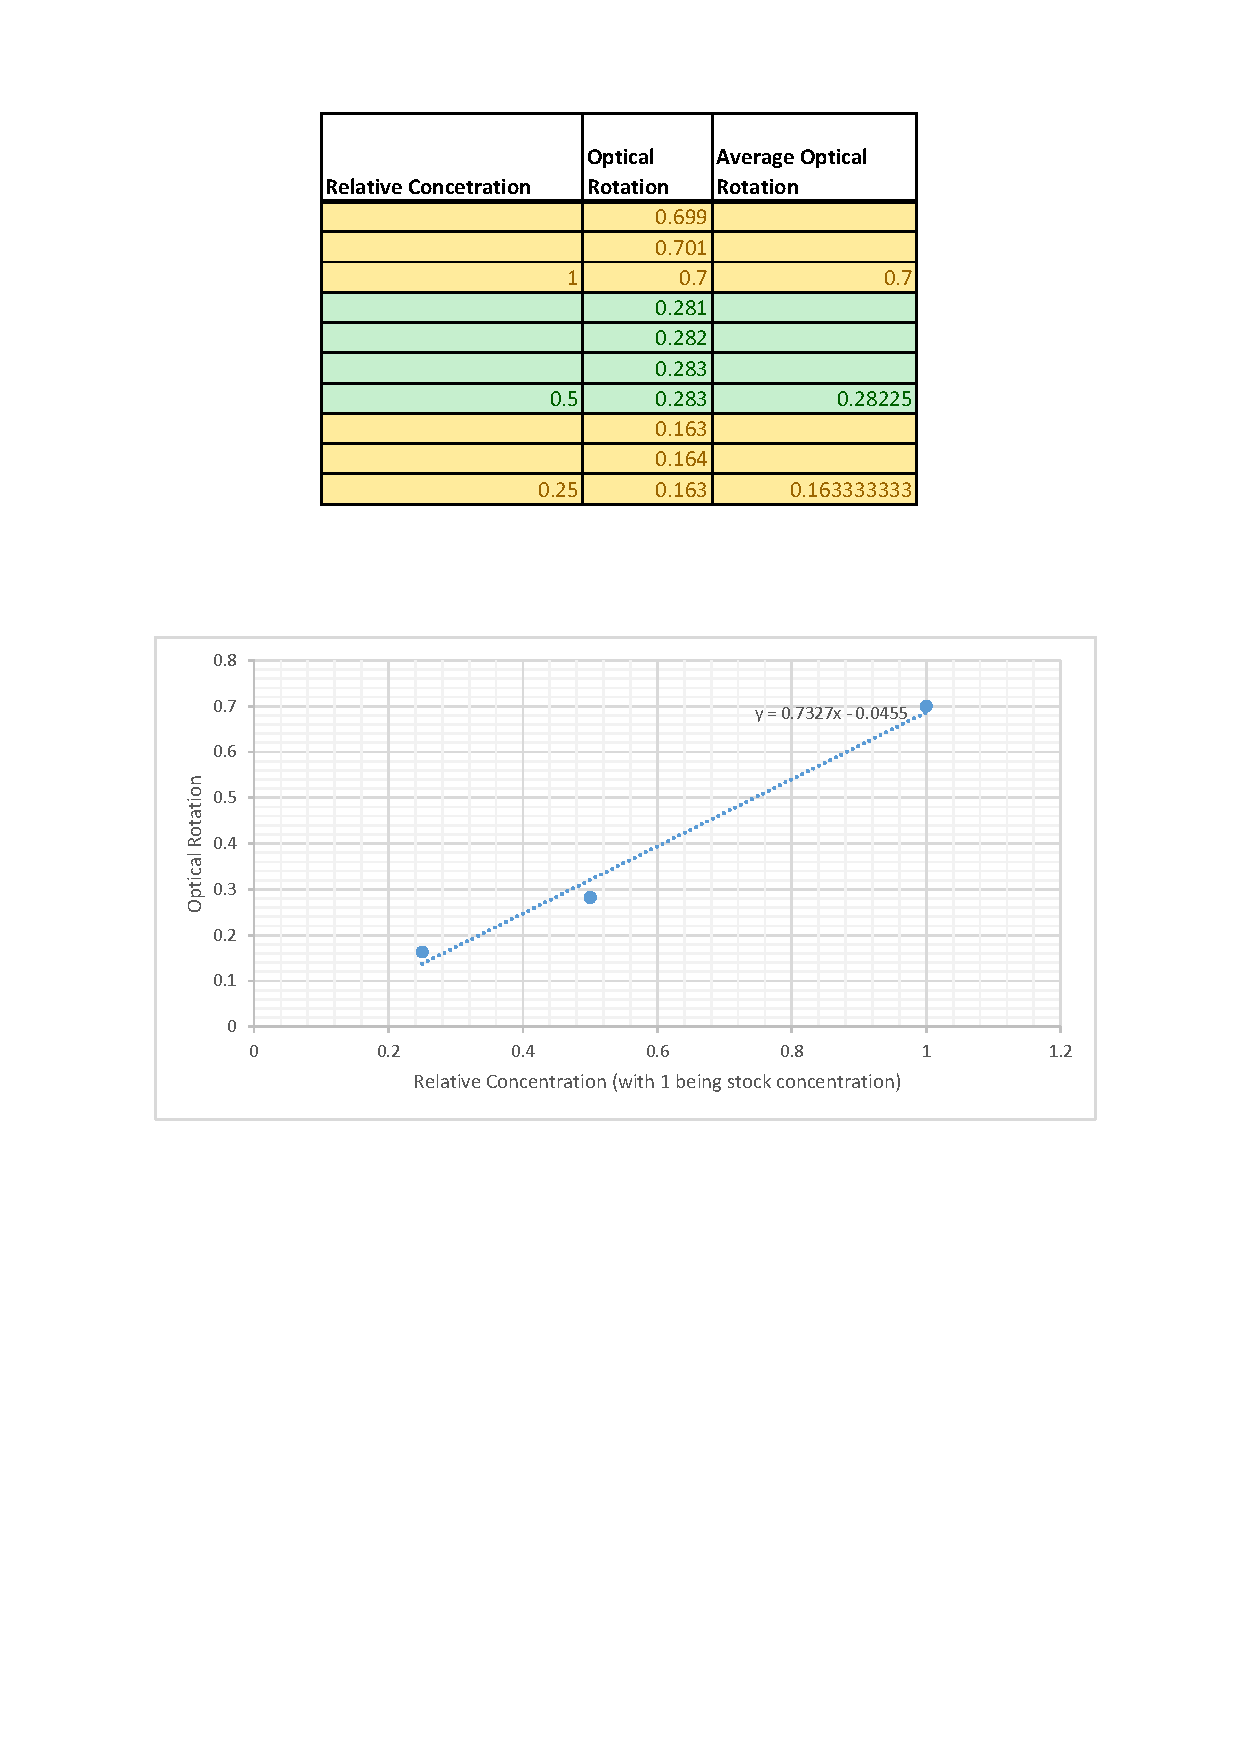
\includegraphics[width=1.15\linewidth]{gfx/11_optical}
			\end{center}
		\caption[Optical Rotation]{\label{E11_optical}}
		\end{figure}

\section{Acknowledgements}
I thank our PhD assistant who performed the experiment for us, and of course Prof. KS Viswanathan for the rest.

\section{References}
	\begin{enumerate}
		\item Prof. K S Viswanathan's Lectures
	\end{enumerate}